\section{Governing equations}\label{model} 
We consider an inviscid fluid disc of mass $M_d$ 
orbiting a central star of mass $M_*$. We will mainly examine 2D
(or razor-thin) discs in favour of numerical 
resolution, but have also carried out some 3D disc
simulations. Hence, for generality we describe the system in
3D, using both cylindrical $(R,\phi,z)$ and spherical polar
coordinates $(r,\theta,\phi)$ centred on the star. 
The governing fluid equations in 3D are  
\begin{align}
  &\frac{\p\rho}{\p t} + \nabla\cdot\left(\rho\bm{v}\right) =
  0,\label{cont_eq}\\
  &\frac{\p\bm{v}}{\p t} + \bm{v}\cdot\nabla\bv = -\frac{1}{\rho}\nabla
  p -\nabla \Phi_\mathrm{tot}\label{mom_eq},\\ 
  & \nabla^2\Phi_d = 4 \pi G \rho \label{poisson}, 
\end{align}
where $\rho$ is the mass density, $\bm{v}$ is the 
fluid velocity (the angular velocity being $\Omega \equiv v_\phi/R$), 
$p$ is the pressure and the total potential
$\Phi_\mathrm{tot} = \Phi_* + \Phi_d$ consists of that from the
central star, 
\begin{align}
  \Phi_*(r) = -\frac{GM_*}{r}, 
\end{align}
where $G$ is the gravitational constant,  and the disc potential
$\Phi_d$. We impose a locally isothermal equation of state 
\begin{align}
  p = c_s^2(R)\rho,
\end{align}
where the sound-speed $c_s$ is given by 
\begin{align}\label{sound-speed}
  % c_s(R) = hR_0\Omega_k(R_0)\left(\frac{R}{R_0}\right)^{-q/2}, 
  c_s(R) = c_{s0}\left(\frac{R}{R_0}\right)^{-q/2}
\end{align}
where $c_{s0} = h R_0\Omega_k(R_0)$ and 
$h$ is the disc aspect-ratio at the reference radius $R=R_0$, 
$\Omega_k=\sqrt{GM_*/R^3}$ is the midplane Keplerian frequency, and
$q$ is the imposed temperature gradient since, for an ideal gas the
temperature is proportional to $c_s^2$. {\bf For convenience we will
  refer to $c_s^2$ as the disc temperature.} The vertical disc scale-height is
defined by $H=c_s/\Omega_k$. Thus, a strictly isothermal disc with
$q=0$ has $H\propto R^{3/2}$, and $q=1$ corresponds to a 
 disc with constant $H/R$. 



The 2D disc equations are obtained by replacing $\rho$ with the surface
mass density $\Sigma$, $p$ becomes the vertically-integrated pressure, 
and the 2D fluid velocity $\bm{v}$ is evaluated at the midplane, as are
the forces in the momentum equations. In the Poisson equation, $\rho$ is
replaced by $\Sigma\delta(z)$, where $\delta(z)$ is the
delta function. 



\section{Linear density waves}\label{wkb}

{\bf We describe a key feature of locally isothermal discs that
  enables angular momentum exchange between small disturbances and the
  background disc through an imposed radial temperature gradient. This
  conclusion results from the consideration of angular momentum
  conservation within the framework of linear perturbation theory. 
  For simplicity, in this section we consider 2D discs. 
}

In a linear analysis, one assumes a steady axisymmetric background state, 
which is then perturbed such that
\begin{align}  
  \Sigma \to \Sigma(R) + \delta\Sigma_m(R)\exp{\left[\ii\left(-\sigma t +
        m\phi\right)\right]}, 
\end{align}
and similarly for other variables, where $\sigma=\omega+\ii\gamma$ is
a complex frequency with $\omega$ being the real frequency, 
$\gamma$ the growth rate, and $m$ is an integer. We take $m>0$ without
loss of generality.  


The linearised mass and momentum equations are
\begin{align}
  &-\ii\sbar \delta\Sigma_m = -\frac{1}{R}\frac{d}{dR}\left(R\Sigma\delta
    v_{Rm}\right) - \frac{\ii m \Sigma}{R}\delta v_{\phi m}, \\
  &-\ii\sbar\delta v_{Rm} - 2\Omega \delta v_{\phi m} = -
  c_s^2(R)\frac{d}{dR}\left(\frac{\delta\Sigma_m}{\Sigma}\right) - \frac{d}{dR}\delta\Phi_m,\label{radmom}\\
  & -\ii\sbar\delta v_{\phi m} + \frac{\kappa^2}{2\Omega}\delta v_{Rm} =
  -\frac{\ii m }{R}\left(c_s^2\frac{\delta\Sigma_m}{\Sigma} + \delta\Phi_m\right),
\end{align}
where $\sbar = \sigma - m\Omega$ and $\kappa^2 =
R^{-3}\p_R(R^4\Omega^2)$ is the square of the epicyclic frequency. A
locally isothermal equation of state has been assumed in
Eq. \ref{radmom}.  The linearised Poisson equation is 
\begin{align}
  \nabla^2\delta\Phi_m = 4\pi G \delta\Sigma_m \delta(z). 
\end{align}

These linearised equations can be combined into a single
integro-differential equation eigenvalue problem. We defer a full
{\bf numerical} exploration of the linear problem to a future study. Here, we {\bf
  discuss} some
general properties of the linear perturbations. 

\subsection{Global angular momentum conservation for linear
  perturbations} \label{global_cons}
It can be shown that linear perturbations with $\phi$-dependence in the form
$\exp{(\ii m\phi)}$ satisfies angular momentum conservation
in the form 
\begin{align}\label{angcons}
  \frac{\p \jlin}{\p t} + \nabla\cdot\bm{F} = \tbg, 
\end{align}
\citep[e.g.][]{narayan87,ryu92,lin93b} where
\begin{align}\label{lin_ang_mom_cons}
  \jlin \equiv
  -\frac{m\Sigma}{2}\imag\left(\bm{\xi}^*\cdot\frac{\p\bm{\xi}}{\p
      t} + \Omega \hat{\bm{k}}\cdot\bm{\xi}\times\bm{\xi}^* + \ii
    m \Omega |\bm{\xi}|^2\right) 
\end{align}
is the angular momentum density of the linear disturbance (which may
be positive or negative), $\bm{\xi}$ is the Lagrangian
displacement and $^*$ denotes complex conjugation, and $\bm{F}$ is the
vertically-integrated angular momentum flux consisting of a Reynolds
stress and a gravitational stress \citep{lin11b}. Explicit expressions
for $\bm{\xi}$ can be found in, e.g. \cite{papaloizou85}. 

In Eq. \ref{angcons}, the background torque density $\tbg$ is 
\begin{align}\label{baroclinic_torque}
  \tbg \equiv
  -\frac{m}{2}\imag\left(\delta\Sigma_m\xi_R^*\frac{dc_s^2}{dR}\right), 
\end{align}
and arises because we have adopted a locally isothermal equation of
state {\bf in the perturbed disc}. {\bf  We outline the
derivation of $T_\mathrm{BG}$ in Appendix \ref{tbg_deriv}.} 

In a barotropic fluid, such as a strictly isothermal disc,
$\tbg$ vanishes and the total angular momentum associated with
the perturbation is conserved, provided that there is no net angular
momentum flux. However, as noted in \cite{lin11b}, if there is an imposed
temperature gradient, as in the disc models we consider,
then $\tbg\neq 0$ in general, which corresponds to a local torque
exerted by the background disc on the perturbation. 

The important consequence of the background torque is the possibility
of instability if $\tbg\jlin>0$. That is, if $\jlin$ is positive
(negative) and the background torque $\tbg$ is {\bf also} positive (negative),
then the local angular momentum density of the linear disturbance
{\bf will} further increase (decrease) {\bf with time}. This implies the amplitude of the disturbance
may grow by exchanging angular momentum with the background
disc.

{\bf 
  We demonstrate instability for low-frequency modes 
  ($|\omega|\ll m\Omega$) by explicitly showing its 
  angular momentum density 
  $\jlin<0$, and the background torque $T_\mathrm{BG}<0$ for
  appropriate perturbations and radial temperature gradients. 
}

\subsection{Angular momentum density of  non-axisymmetirc low-frequency modes}
From Eq. \ref{lin_ang_mom_cons} and assuming a time-dependence of the
form $\exp{(-\ii \sigma t)}$ with $\real{\sigma} = \omega$,  
the angular momentum density associated with linear waves is
\begin{align}
  \jlin = \frac{m\Sigma}{2}\left[\left(\omega -
      m\Omega\right)|\bm{\xi}|^2 + \ii\Omega\left(\xi_R\xi_\phi^* -
      \xi_R^*\xi_\phi\right)\right].\label{ang_mom_def}  
\end{align}
For a low-frequency mode, $|\omega|\ll m\Omega$. Then neglecting the
term $\omega|\bm{\xi}|^2$, {\bf we find}
\begin{align}
  \jlin &\simeq \frac{m\Sigma\Omega}{2}\left[-m|\bm{\xi}|^2 + \ii\left(\xi_R\xi_\phi^* -
      \xi_R^*\xi_\phi\right)\right]\notag\\
  & = -\frac{m\Sigma\Omega}{2}\left[ (m-1)|\bm{\xi}|^2 +  |\xi_R + \ii\xi_\phi|^2\right].
%  & \leq 0.
\end{align}
{\bf
Thus, non-axisymmetric ($m\geq1$) low-frequency modes generally have 
negative angular momentum. If the mode loses (positive) angular momentum 
to the background, then we can expect instability. We show 
below how this is possible through a forced temperature
gradient via the background torque. It is simplest to calculate
$T_\mathrm{BG}$ in the local approximation, which we review first.  
}

%and setting $m=1$,
%\begin{align}
 % \jlin &\simeq \frac{\Sigma\Omega}{2}\left[-|\bm{\xi}|^2 + \ii\left(\xi_R\xi_\phi^* -
  %    \xi_R^*\xi_\phi\right)\right]\notag\\
%  & = -\frac{\Sigma\Omega}{2}|\xi_R + \ii\xi_\phi|^2\notag\\
 % & \leq 0.
%\end{align}

\subsection{Local results}\label{local_approx}
In the local approximation, perturbations are assumed to vary rapidly
relative to any background gradients. The
dispersion relation for tightly-wound density 
waves of the form $\exp{[\ii(-\sigma t + m \phi + kR)]}$ in a razor-thin
disc is  
\begin{align}\label{dispersion}
  (\sigma - m\Omega)^2 = \kappa^2 + k^2c_s^2 - 2\pi G \Sigma |k|, 
\end{align}
where $k$ is a real wavenumber such that $|kR|\gg1$ \citep{shu91}. 
Note that in the {\bf strictly} local approximation, {\bf where all
  global effects are neglected}, only axisymmetric perturbations
($m=0$) can be unstable. % (having an imaginary $\sigma$).     

Given the real frequency $\omega$ or pattern speed $\Omega_p\equiv  
\omega/m$ of a {\bf non-axisymmetric} neutral mode 
, Eq. \ref{dispersion} can be solved 
for $|k|$, 
\begin{align}\label{wavenumber}
%  |k| = \frac{\pi G \Sigma}{c_s^2}\left[1 \pm \sqrt{1 -
 %     Q^2(1-\nu^2)}\right], 
|k| = k_c\left[1 \pm \sqrt{1 -
     Q^2(1-\nu^2)}\right], 
\end{align}
where 
 \begin{align}
   k_c \equiv \frac{\pi G \Sigma}{c_s^2}
 \end{align}
 is a characteristic wavenumber, 
\begin{align}
  Q \equiv \frac{c_s\kappa}{\pi G \Sigma}
\end{align}
is the usual Toomre parameter, and
\begin{align}
  \nu \equiv \frac{(\omega - m\Omega)}{\kappa}
\end{align}
is a dimensionless frequency. In
Eq. \ref{wavenumber}, the upper (lower) sign correspond to short
(long) waves, and $k>0$ ($k<0$) correspond to trailing (leading)
waves.    

{\bf At the \emph{co-rotation radius} $R_c$} the pattern speed matches
the fluid rotation,
\begin{align}
  \Omega(R_c) = \Omega_p.
\end{align}
\emph{Lindblad resonances} $R_L$ occurs where
\begin{align}
  \nu^2(R_L) = 1. 
\end{align}
Finally, \emph{Q-barriers} occur at radii $R_{Qb}$ where
\begin{align}
  Q^2(R_{Qb})\left[1-\nu^2(R_{Qb})\right] = 1.  
\end{align}
According to Eq. \ref{wavenumber}, purely wave-like solutions with
real $k$ are only possible where $Q^2(1-\nu^2)\leq1$.  

A detailed discussion of the properties of local density waves 
is given in \cite{shu91}. An important result, {\bf which holds for
  waves of all frequencies}, is that
waves interior to co-rotation ($R<R_c$) have negative angular momentum, while
waves outside co-rotation ($R>R_c$) have positive angular
momentum. 

\subsection{Unstable interaction between low-frequency modes 
  and the background disc due to an imposed temperature gradient}
{\bf 
Here we show that the torque density acting on a low-frequency, 
local mode due to the background temperature gradient can be negative, which 
would enforce the mode, because it has negative angular momentum.  
}

The Eulerian surface density perturbation is given by
\begin{align}\label{den_pert}
  \delta\Sigma_m = -\nabla\cdot\left(\Sigma\bm{\xi}\right) 
  = -\frac{1}{R}\frac{d}{dR}\left(R\Sigma \xi_R\right) - \frac{\ii m}{R}\Sigma\xi_\phi.  
\end{align}
We invoke local theory by setting $d/dR \to \ii k$ where $k$ is
real, and assume $|kR|\gg m$ so that the second term on the right hand
side of Eq. \ref{den_pert} can be neglected. Then    
\begin{align}
  \delta\Sigma _m  \simeq -\ii k \Sigma \xi_R.
\end{align}
{\bf Inserting this into the expression for the background torque,
  Eq. \ref{baroclinic_torque}, we find}
\begin{align}
  T_\mathrm{BG} = \frac{m}{2}\frac{dc_s^2}{dR}k\Sigma |\xi_R|^2. \label{baroclinic_torque1}
\end{align}


This torque density is negative for trailing waves ($k>0$) in discs with
a fixed temperature profile decreasing outwards ($dc_s^2/dR<0$). Note
that this conclusion does not rely on the low-frequency approximation.    

However, if the linear disturbance under consideration \emph{is} a
low-frequency mode, then it has negative angular
momentum. If it is trailing and $dc_s^2/dR<0$, as is typical
in astrophysical discs, then $T_\mathrm{BG}<0$ and
the background disc applies a negative torque on the disturbance,
which further decreases its angular momentum. This suggests the {\bf
  mode} 
amplitude will grow.  

Using $\jlin$ and $T_\mathrm{BG}$, we can estimate the 
growth rate $\gamma$ of linear perturbations due to the background
torque as  
\begin{align}
  2\gamma \sim \frac{T_\mathrm{BG}}{\jlin},
\end{align}
where the factor of two accounts for the fact that the angular momentum
density is quadratic in the linear perturbations. Inserting the above
expressions for $\jlin$ and $T_\mathrm{BG}$ for gives
\begin{align}\label{theoretical_rate0}
  2\gamma \sim
  -\frac{dc_s^2}{dR}
  \frac{k}{\Omega}\frac{|\xi_R|^2}{\left[(m-1)|\bm{\xi}|^2 + |\xi_R +
      \ii\xi_\phi|^2 \right]} 
  = -\frac{dc_s^2}{dR}
  \frac{k}{m\Omega},
%  -\frac{dc_s^2}{dR}\frac{k}{\Omega}\frac{|\xi_R|^2}{|\xi_R + \ii
%   \xi_\phi|^2}. 
\end{align}
{\bf where the second equality uses $\xi_\phi \simeq
2\ii \xi_R/m$ in the local approximation, as shown in  Appendix
\ref{horizontal_displacements}.} 
Then for the temperature profiles $c_s^2 = c_{s0}^2 (R/R_0)^{-q}$ as
adopted in our disc models,  
\begin{align}
  2\gamma \sim q\frac{c_s^2}{R}\frac{k}{m\Omega} \sim q h
  \left(\frac{kH}{m}\right)\Omega,\label{theoretical_rate}
\end{align}
where we used $c_s\sim H\Omega\sim hR\Omega$. {\bf
  Eq. \ref{theoretical_rate} suggests that perturbations with small
  radial length-scales ($kH\gtrsim m$) are most favourable for
  destabilisation. Taking the local approximation is then
  appropriate.}       


{\bf Note that the derivation of Eq. \ref{baroclinic_torque1} and 
  Eq. \ref{theoretical_rate} do not 
  require the disc to be self-gravitating. Thus, destabilisation by the
  background torque is not directly associated with disc
  self-gravity. However, in order to evaluate 
  Eq. \ref{baroclinic_torque1} or Eq. \ref{theoretical_rate} in terms 
  of disc parameters (as done in \S\ref{fargo_m1}), we need to insert a 
  value of $k$, which may depend on disc    
  self-gravity (e.g. from Eq. \ref{wavenumber}).  
}   


\section{Numerical simulations}\label{methods}

{\bf
  We demonstrate the destabilising effect of a fixed temperature
  gradient using numerical simulations. The above discussion is
  generic for low-frequency non-axisymmetric modes, but for
  simulations we will consider specific examples.  
  
  There are two parts to the destabilising mechanism: 
  the disc should support low-frequency modes, which is then
  destabilised by an imposed temperature gradient. The latter is
  straight forward to implement by adopting a locally isothermal
  equation of state as described in \S\ref{model}.  For the former, we
  consider discs with a  
  radially-structured Toomre $Q$ profile. We use local theory to show
  that such discs can trap 
  low-frequency one-armed ($m=1$) modes.  
  This is convenient because Eq. \ref{theoretical_rate} indicates that
  modes with small $m$ are
  more favourable for destabilisation. 
}


\subsection{Disc model and initial conditions}
For the initial disc profile we adopt a modified power-law disc with
surface density given by
\begin{align}
  \Sigma(R) = \Sigma_\mathrm{ref} \left(\frac{R}{R_0}\right)^{-s}\times B(R;
  R_{1}, R_{2}, \epsilon, \delta R), 
\end{align}
where $s$ is the power-law index describing the smooth disc and
$\Sigma_\mathrm{ref}$ is a 
surface density scale chosen by specifying $Q_\mathrm{out}$,
the Keplerian Toomre parameter at $R=R_{2}$,
\begin{align}
  Q_\mathrm{out} = \left.\frac{c_s\Omega_k}{\pi G
    \Sigma}\right|_{R=R_{2}}. 
\end{align}
The bump function
$B(R)$ represents a surface density boost between
$R\in[R_{1},R_{2}]$ by a factor $\epsilon^{-1}>1$,
and $\delta R$ is the transition width between the bump and the
smooth disc. We choose 
\begin{align}\label{sig_bump}
  &B(R) = f_1(R)\times f_2(R),\\
  &f_1(R) = \frac{1}{2}\left(1 - \epsilon\right)\left[1 +
    \tanh\left(\frac{R-R_{1}}{\Delta_1}\right)\right]  + \epsilon,\\
  &f_2(R) = \frac{1}{2}\left(1 - \epsilon\right)\left[1 -
    \tanh\left(\frac{R-R_{2}}{\Delta_2}\right)\right]  + \epsilon,
\end{align}
where $\Delta_{1,2} = \delta R \times H(R_{1,2})$. 

The 3D disc structure is obtained by assuming vertical hydrostatic
balance  
\begin{align}
  0 = \frac{1}{\rho}\frac{\p p}{\p z} + \frac{\p\Phi_*}{\p z} + \frac{\p
    \Phi_d}{\p z},  
\end{align}
which gives the mass density as 
\begin{align}
  \rho = \frac{\Sigma}{\sqrt{2\pi}H}Z(R,z),
\end{align}
where $Z(R,z)$ describes vertical stratification. In practice, we
numerically solve for $Z(R,z)$ by neglecting the radial self-gravity
force compared to vertical self-gravity, which reduces the equations
for vertical hydrostatic equilibrium to ordinary differential
equations. This procedure is described in \cite{lin12b}. 

Our fiducial parameter values are: $s=2$, $R_{1}=R_0$, $R_{2}=2R_0$,
$\epsilon=0.1$, $\delta R=5$, $h=0.05$ and
$Q_\mathrm{out}=2$. An example of the initial surface density and the
Toomre $Q$ parameter is shown in
Fig. \ref{initial_surf}. Since $Q>1$, the disc is stable to local
axisymmetric perturbations \citep{toomre64}. %min Q is 1.3
The transition between self-gravitating and 
non-self-gravitating portions of the disc occur smoothly across
$\sim10H$. Initially there is no vertical or radial velocity
($v_R = v_r = v_\theta = 0$). The azimuthal velocity is initialized to
satisfy centrifugal balance with pressure and gravity,
\begin{align}
  \frac{v_\phi^2}{r} = \frac{1}{\rho}\frac{\p p}{\p r} + \frac{\p
    \Phi_\mathrm{tot}}{\p r}
\end{align}
and similarly in 2D.  

\begin{figure}
  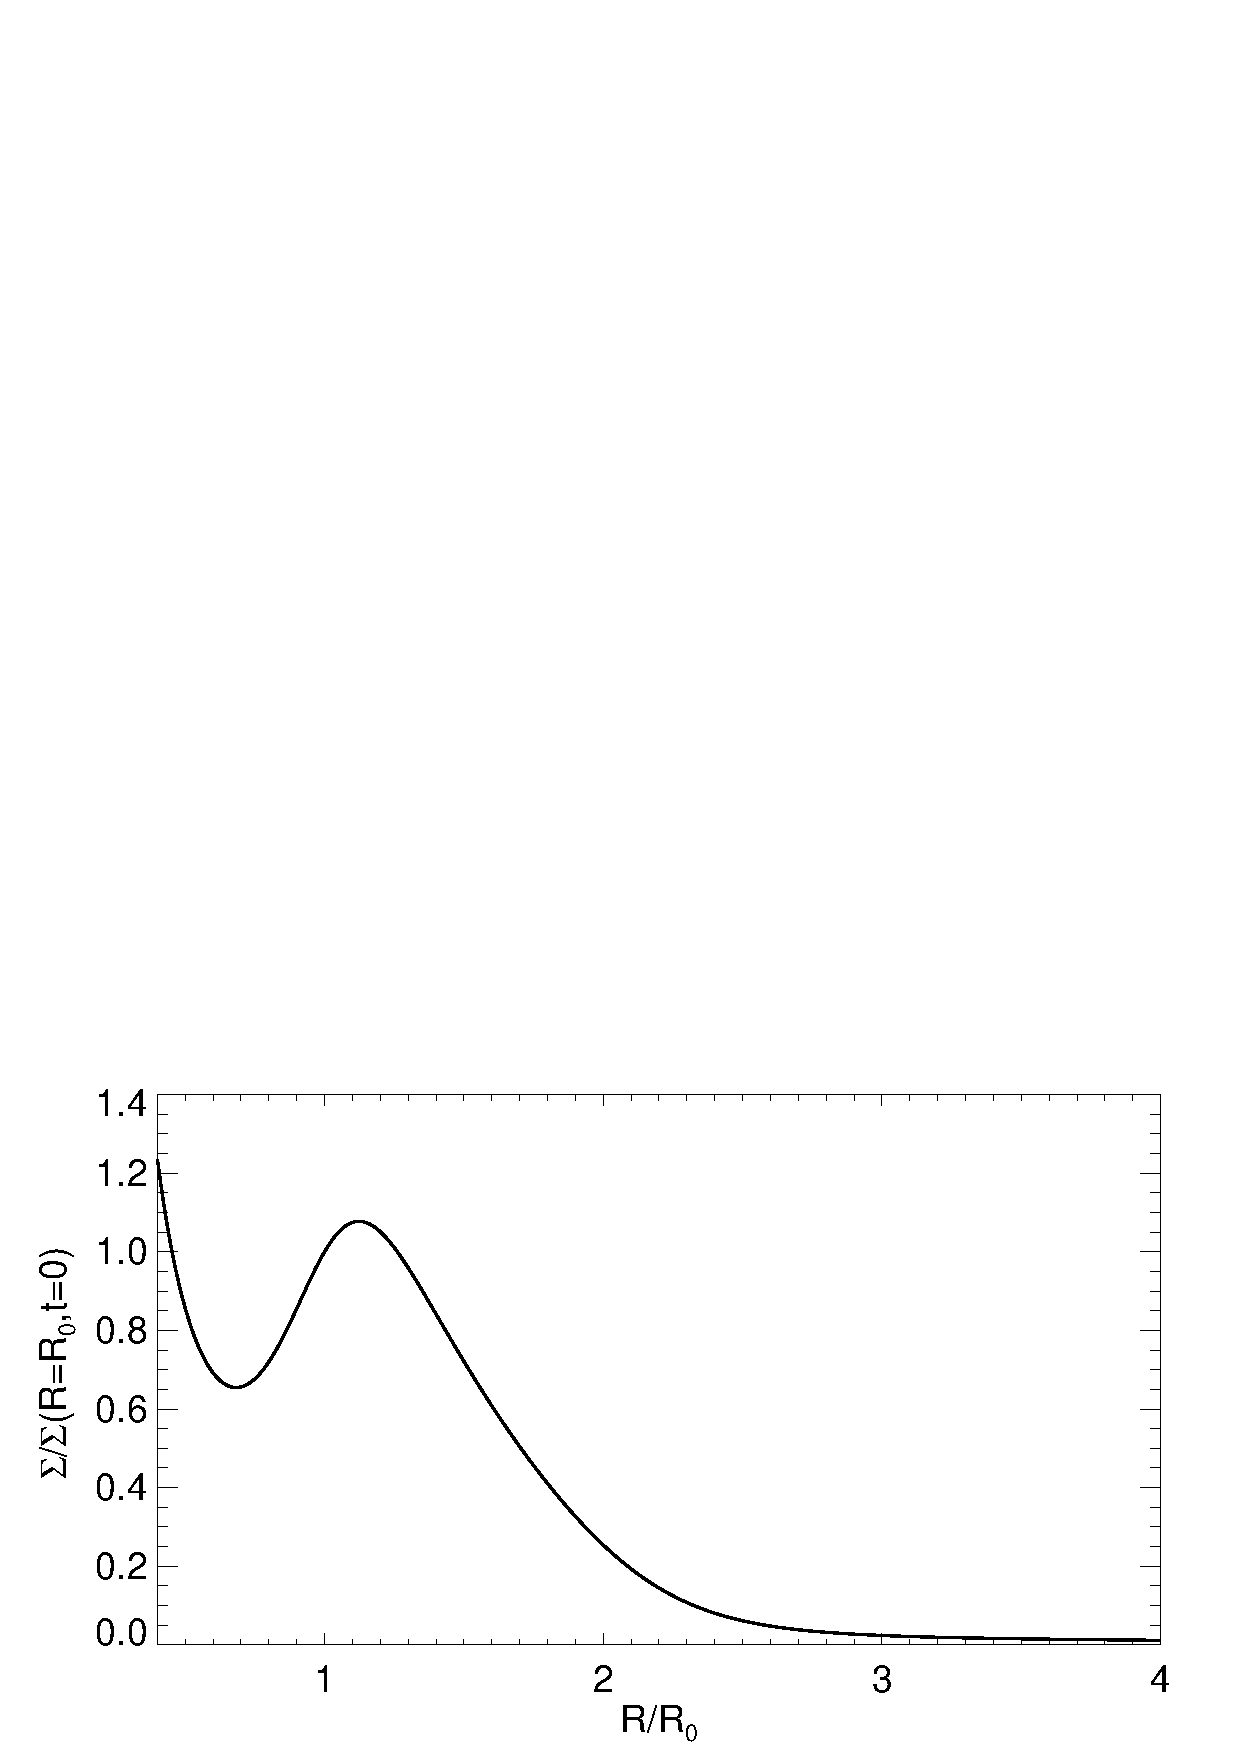
\includegraphics[width=\linewidth,clip=true,trim=0cm 1.7cm 0cm
  0cm]{figures/compare_profiles_dens000} 
  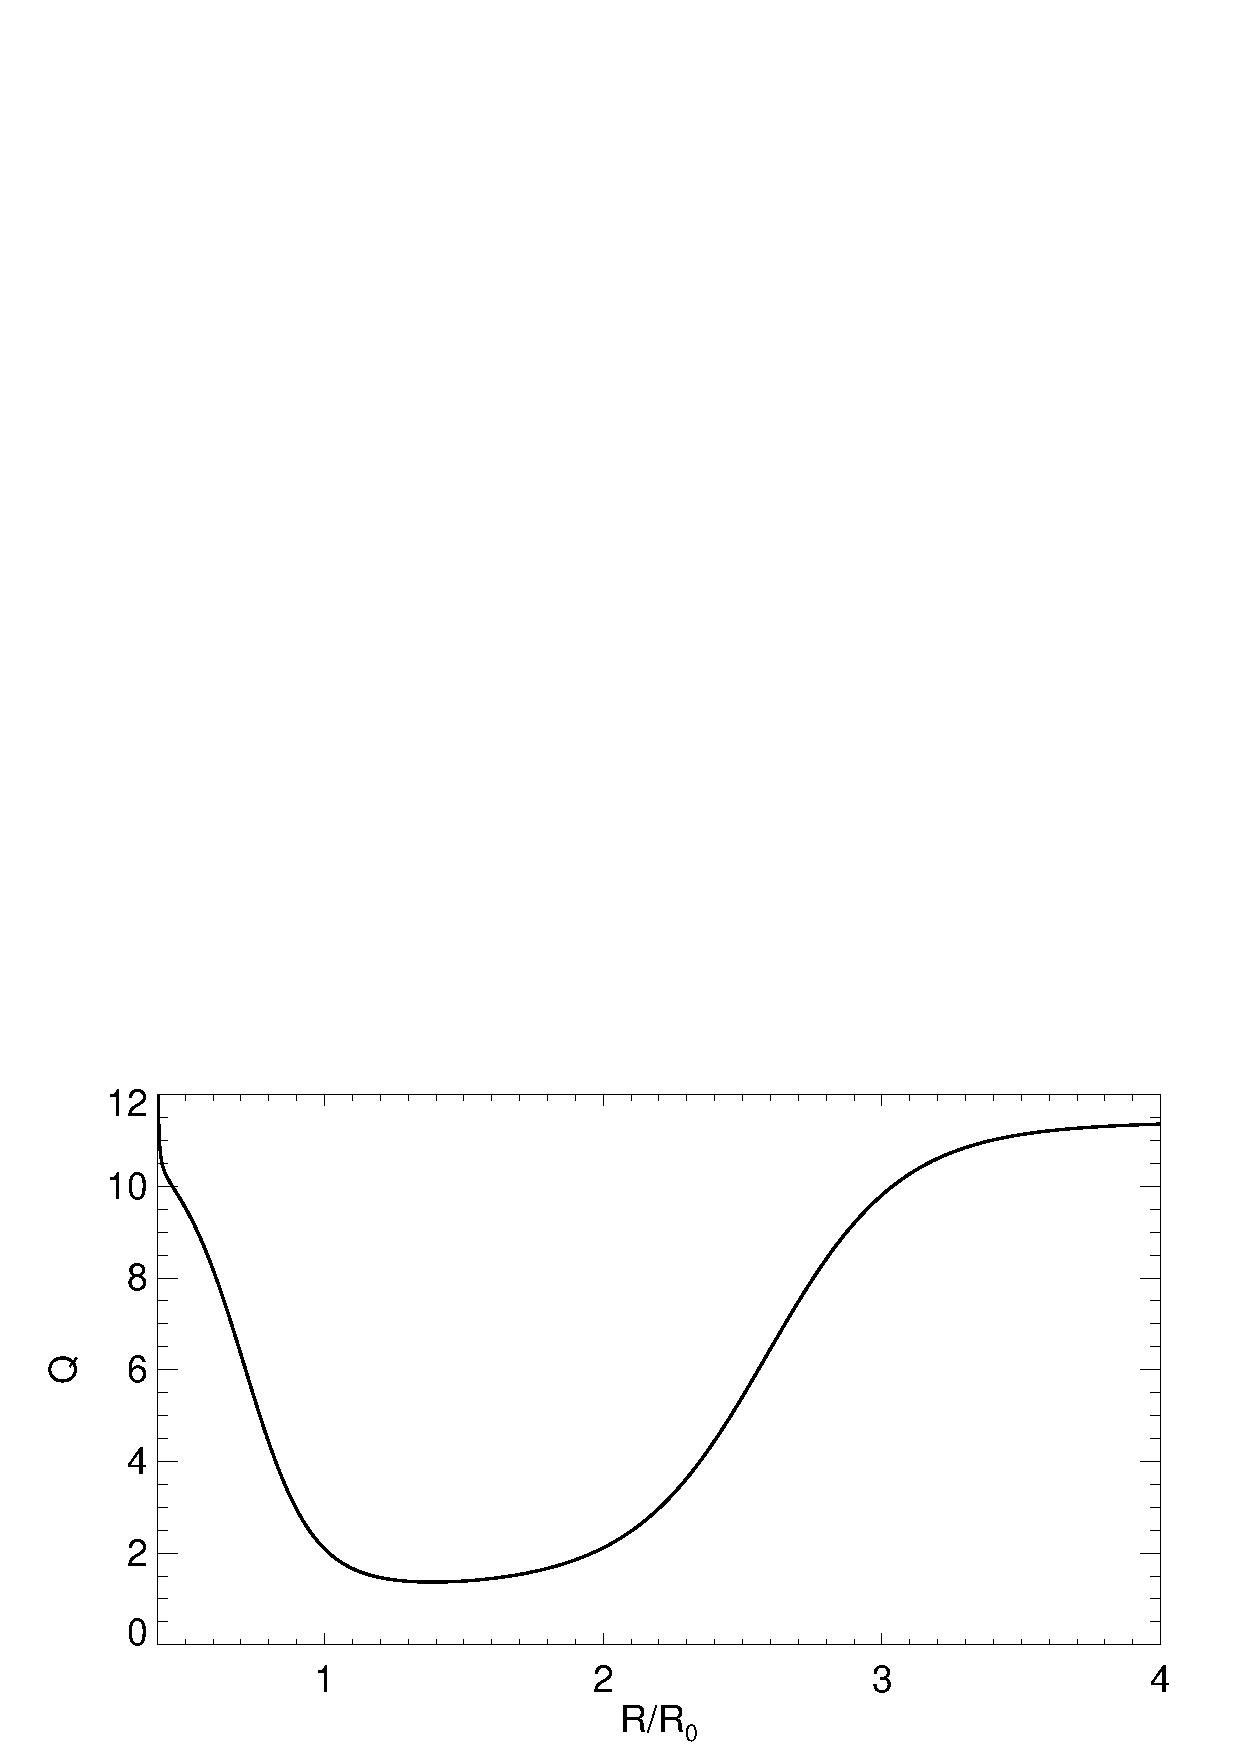
\includegraphics[width=\linewidth]{figures/compare_profiles_Q000}
  \caption{Fiducial profiles of the surface density (top) and Toomre
    parameter (bottom) used in this work.\label{initial_surf}}
\end{figure}

\subsection{Codes}
{\bf We use three independent grid-based codes to simulate the above 
system.} We adopt computational units such that
$G=M_*=R_0=1$. Time is measured  in the Keplerian orbital period at
the reference radius, $P_0\equiv  2\pi/\Omega_k(R_0)$.   

\subsubsection{FARGO}
Our primary code is FARGO with self-gravity \citep{baruteau08}. This
is a popular, simple finite-difference code for 2D discs. `FARGO' refers
to its azimuthal transport algorithm, which removes the mean azimuthal
velocity of the disc, thereby permit larger timesteps than that would otherwise be allowed
by the usual Courant condition based on the full azimuthal
velocity \citep{masset00a,masset00b}.     

The 2D disc occupies
$R\in[R_\mathrm{min},R_\mathrm{max}],\,\phi\in[0,2\pi]$ and is  
divided into $(N_R,N_\phi)$ grids, logarithmically spaced in radius and
uniformly spaced in azimuth. At radial boundaries we set the
hydrodynamic variables to their initial values.   

The 2D Poisson equation is solved in integral form, 
\begin{align}\label{2d_grav}
  &\Phi_{d,z=0}(R,\phi) \notag \\
  &=-\int_{R_\mathrm{min}}^{R_\mathrm{max}} \int_0^{2\pi}
  \frac{G\Sigma(R^\prime,\phi^\prime)R^\prime dR^\prime d\phi^\prime}{\sqrt{R^2+R^{\prime 2} -
      2RR^\prime\cos{(\phi - \phi^\prime)} + \epsilon_g^2}}, 
\end{align}
using Fast Fourier Transform (FFT), where $\epsilon_g$ is a softening
length to prevent a numerical singularity. The FFT approach requires
$\epsilon_g\propto R$ \citep{baruteau08}. In FARGO, $\epsilon_g$ is
set to a fraction of $hR$.  

\subsubsection{ZEUS-MP}
ZEUS-MP  is a general-purpose finite difference
code \citep{hayes06}. We use the code in 3D spherical geometry, covering
$r\in[r_\mathrm{min},r_\mathrm{max}]$, $\theta\in[\theta_\mathrm{min},\pi/2]$,
$\phi\in[0,2\pi]$. The vertical domain is chosen to cover $n_H$
scale-heights at $R=R_0$, i.e. $\tan{(\pi/2 - \theta_\mathrm{min})}/h=n_H$. 
The grid is logarithmically spaced in radius and uniformly spaced in the angular
coordinates. We assume symmetry across the midplane, and
apply reflective boundary conditions at radial boundaries and the
upper disc boundary.  

ZEUS-MP solves the 3D Poisson equation using a conjugate gradient
method. To supply boundary conditions to the linear solver, we
expand the boundary potential in spherical harmonics $Y_{lm}$ 
as described in \cite{boss80}. The expansion is truncated at
$(l,m)=(\lmax,\mmax)$. This code was used in \cite{lin12b} for
self-gravitating disc-planet simulations.  

\subsubsection{PLUTO} 
PLUTO is a general-purpose Godunov code \citep{mignone07}. The grid
setup is the same as that adopted in ZEUS-MP above. We configure the
code similarly to that used in \cite{lin14}: piece-wise linear
reconstruction, a Roe solver and second order Runge-Kutta time
integration. We also enable the FARGO algorithm for azimuthal
transport. 

We solve the 3D Poisson equation throughout the domain using spherical
harmonic expansion \citep{boss80}, as used for the boundary potential
in ZEUS-MP. This version of PLUTO was used in \cite{lin14b} for
self-gravitating disc-planet simulations, producing similar results to
that of ZEUS-MP and FARGO.   

\subsection{Diagnostics}

\subsubsection{Evolution of non-axisymmetric modes}
The disc evolution is quantified using mode amplitudes and angular
momenta as follows. We list the 2D definitions with obvious 3D generalisations. 
A hydrodynamic variable $f$ (e.g. $\Sigma$) is written as 
\begin{align}
  f(R,\phi,t) &= \sum_{m=-\infty}^{\infty}f_m(R,t)\exp{\ii m \phi} \notag\\
  &= f_0 + 2 \real\left[\sum_{m=1}^\infty f_m \exp{(\ii
      m\phi)}\right], 
\end{align}
where the $f_m$ may be obtained from Fourier transform in $\phi$. 

The normalised surface density with azimuthal wavenumber $m$ is
\begin{align}
  \Delta\Sigma_m = \frac{2}{\Sigma_{00}} \real\left[\Sigma_m \exp{(\ii
      m\phi)}\right]
\end{align}
where $\Sigma_{00} = \Sigma_0(t=0)$. The time evolution of the
$m^\mathrm{th}$ mode can be characterized by 
assuming $\Sigma_m\propto\exp{(-\ii \sigma t)}$ as in linear
theory. 

The total non-axisymmetric surface density is 
\begin{align}
  \Delta\Sigma = \frac{\Sigma - \Sigma_0}{\Sigma_0}. 
\end{align}

\subsubsection{Angular momentum decomposition}
The total disc angular momentum is
\begin{align}
  J &= \int_{R_\mathrm{min}}^{R_\mathrm{max}}\int_0^{2\pi} \Sigma Rv_\phi RdRd\phi \notag\\
  &= 2\pi\int_{R_\mathrm{min}}^{R_\mathrm{max}} R\Sigma_0 v_{\phi0} R dR \notag\\ 
  &\phantom{=}+
  \sum_{m=1}^\infty2\pi\int_{R_\mathrm{min}}^{R_\mathrm{max}} 2R\real\left[\Sigma_m v_{\phi
      m}^*\right] RdR 
  = \sum_{m=0}^\infty J_m. 
\end{align}
We will refer to $J_m$ as the
$m^\mathrm{th}$ component of the total angular momentum, and use it to
monitor numerical angular momentum conservation in the simulations. 
It is important to distinguish this empirical definition from the
angular momentum of linear perturbations given in \S\ref{wkb}, which
is defined through a conservation law. 

\subsubsection{Three-dimensionality}
In 3D simulations we measure the importance of vertical motion with
$\Theta$, where 
\begin{align}\label{theta}
  \Theta^2 \equiv \frac{\avg{v_z^2}}{\avg{v_R^2}+\avg{v_\phi^2}}, 
\end{align}
and $\avg{\cdot}$ denotes the density-weighted average, e.g., 
\begin{align}
  \avg{v_z^2} \equiv\frac{
    \int_{R_1}^{R_2}\int_{\theta_\mathrm{min}}^{\pi/2} \int_{0}^{2\pi}
    \rho v_z^2 dV}{
    \int_{R_1}^{R_2}\int_{\theta_\mathrm{min}}^{\pi/2} \int_{0}^{2\pi}
    \rho dV
  },
\end{align}
and similarly for the horizontal velocities. Thus $\Theta$ is the
ratio of the average kinetic energy associated with vertical motion to
that in horizontal motion. The radial range of
integration is taken over $r\in[R_1,R_2]$ since this is where
we find the perturbations to be confined. 


